\experiment{4}{%
    Calculate measure of variablity such as range, variance and standard deviation for a dataset. Interpret what these measure indicate about the spread of the data.
}

\subsection{Calculating measure of variablity}

\subsubsection*{i) Range}

range = max - min

\begin{lstlisting}[style=python]
import pandas as pd 
import matplotlib.pyplot as plt 
import numpy as np

df_student = pd.read_csv("dataset.csv", delimiter=',', header='infer')

minval = df_student[['Marks', 'StudyHours', 'Attendance']].min()
maxval = df_student[['Marks', 'StudyHours', 'Attendance']].max()

rng = pd.DataFrame({
    'Attribute': minval.index,
    'Minimum': minval.values,
    'Maximum': maxval.values,
    'Range': (maxval - minval).values
})

print(rng)
\end{lstlisting}

\textbf{Output:}

\begin{tabular}{ccccc}
    \toprule
    & \textbf{Attribute} & \textbf{Minimum} & \textbf{Maximum} & \textbf{Range} \\
    \midrule
    0 & Marks  & 35 & 95 & 60 \\
    1 & StudyHours  & 1 & 7 & 6 \\
    2 & Attendance  & 42 & 99 & 57 \\
    \bottomrule
\end{tabular}


\subsubsection*{ii) Variance}

\begin{lstlisting}[style=python]
print(df_student[['Marks', 'StudyHours', 'Attendance']].var().round(3))
\end{lstlisting}

\textbf{Output:}

\begin{tabular}{cc}
    \toprule
    Marks  & 345.752 \\
    StudyHours  & 3.995 \\
    Attendance  & 301.357 \\
    \bottomrule
\end{tabular}

\subsubsection*{iii) Standard Deviation}

\begin{lstlisting}[style=python]
df_student[['Marks', 'StudyHours', 'Attendance']].agg(['std', 'mean']).T.round(3)
\end{lstlisting}

\textbf{Output:}

\begin{tabular}{ccc}
    \toprule
    & \textbf{std} & \textbf{mean} \\
    \midrule
    Marks  & 18.594 & 70.200 \\
    StudyHours  & 1.999 & 4.067 \\
    Attendance  & 17.360 & 75.567 \\
    \bottomrule
\end{tabular}

\subsection{Representation}
% histogram with marksing
% box plot  for range
% bar chart of mean with sd on top
\subsubsection*{i) Spread of Marks}

\begin{lstlisting}[style=python]
sturges = round(1+np.log2(df_student.Marks.count()))

mean = df_student.Marks.mean()
std = df_student.Marks.std()

plt.hist(df_student.Marks, ec='white', bins=sturges, zorder=2, label="students")

plt.xlabel('Marks')
plt.ylabel('Frequency')

plt.axvline(mean-std, linestyle='--', color='#F9AA33', label = "mean - std")
plt.axvline(mean, linestyle=':', label = "mean")
plt.axvline(mean+std, linestyle='--', color='#8EBA42', label = "mean + std")

plt.legend()
plt.grid(zorder=0, linestyle=':', alpha=0.6)

plt.show()

\end{lstlisting}

\textbf{Output:}

\begin{figure}[H]
    % \centering
    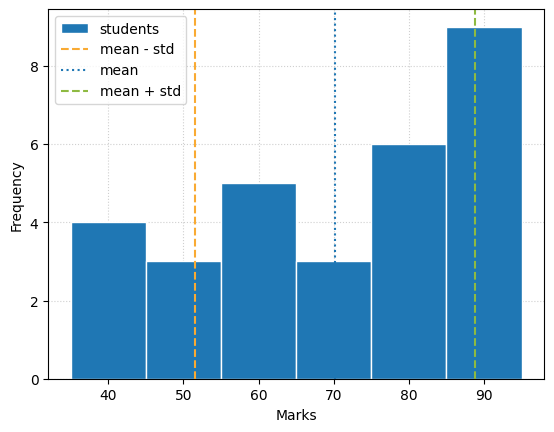
\includegraphics[width=0.75\textwidth]{img/exp4_markHist.png}
    % \caption{Marks of Each Student — Bar Chart}
    % \label{fig:marks_bar}
\end{figure}


\subsubsection*{ii) Majority distribution in each attribute}

\begin{lstlisting}[style=python]
mean = df_student[['Marks', 'StudyHours', 'Attendance']].mean()
std = df_student[['Marks', 'StudyHours', 'Attendance']].std()

plt.errorbar(mean.index, mean.values, std.values, fmt='o', capsize=6, zorder = 2)

plt.grid(zorder=0, linestyle=':', alpha=0.6)
plt.show()

\end{lstlisting}

\textbf{Output:}

\begin{figure}[H]
    % \centering
    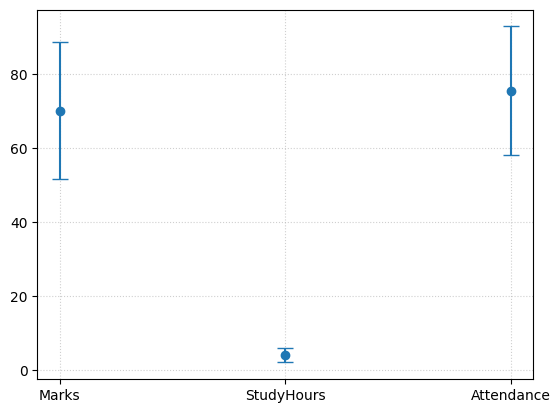
\includegraphics[width=0.75\textwidth]{img/exp4_errorplt.png}
    % \caption{Marks of Each Student — Bar Chart}
    % \label{fig:marks_bar}
\end{figure}



\subsection{Observation}

i. The range of Marks is 60, StudyHours is 6 and Attendance is 57. Marks and Attendance have a wider spread compared to StudyHours.

ii. The standard deviation of Marks is 18.59, meaning most students scored within $\pm$18.59 of the mean, i.e. between 51.6 \& 88.8. This can be seen in graphs above

iii. StudyHours has lowest variance and standard deviation, indicating that study hours is relatively consistent across students compared to thier marks or attendnace.

iv. Attendance has a varaince of 301.36 and standard deviation of 17.36, suggesting some inconsistency in how regular students atteneded class.

v. High standard deviation of marks suggest that class is heterogeneous, i.e. performance varies from student to student.